\chapter{Evaluation Results} \label{chap:evaluation_results}

Following the system's implementation, we needed to evaluate how visualizing the \acf{POP} algorithm in a \ac{VR} environment enhances its learning effectiveness. This chapter presents the results of the evaluation process. We first describe the sample population and the evaluation process. Afterwards, we present the results of the evaluation, which include the participants' feedback and the results of their surveys.

\section{Participants}

We invited 20 participants for the evaluation process. The participants were students from the \acf{MET} program at the \acf{GUC}. All participants had a \ac{CS} background, and were in their third, fourth, or fifth year of study. The ages of the participants ranged from 21 to 25 years old. An important selection criterion was that the participants had no prior knowledge of the \ac{POP} algorithm. This criterion was essential to ensure that the participants' feedback was not biased by their prior knowledge of the algorithm or their practice and experience with it.

\section{Evaluation Process}

The evaluation process was divided into two main parts: an explanation session of the \ac{POP} algorithm and a test session. Since the participants had no prior knowledge of the \ac{POP} algorithm, the explanation session was essential to introduce them to the algorithm and its concepts. The test session was then conducted to evaluate the participants' understanding of the algorithm and their ability to solve problems using it. Finally, the participants were asked to fill out a survey to provide feedback on their experience with the \ac{VR} environment and the \ac{POP} algorithm.

\subsection{Explanation Session}
The explanation session was conducted in a classroom setting, where the participants were introduced to the \ac{POP} algorithm. The session was divided into two parts: a quick theoretical explanation of the algorithm and a theoretical example of the algorithm that is different from the one used in the \ac{VR} environment, but with a similar level of complexity.

\subsection{Test Session}
The test session was conducted in the \ac{VR} environment, where the participants were asked to solve a problem using the \ac{POP} algorithm. The participants were given a brief introduction to the \ac{VR} environment and the controls used to interact with it. The planning problem that the participants were asked to solve was a simplified version of the \textit{Milk, Bananas, and Cordless Drill} problem. The problem is called the \textit{Groceries Buying} problem, and it involves buying groceries from a store and returning home, while keeping in mind the constraints and avoiding the threats. Since the explanation session was a quick explanation to the algorithm, the participants were allowed to ask questions and request clarifications during the test session.
%show some participants in the testing
\begin{figure}[H]
    \centering
    \begin{minipage}{0.45\textwidth}
        \centering
        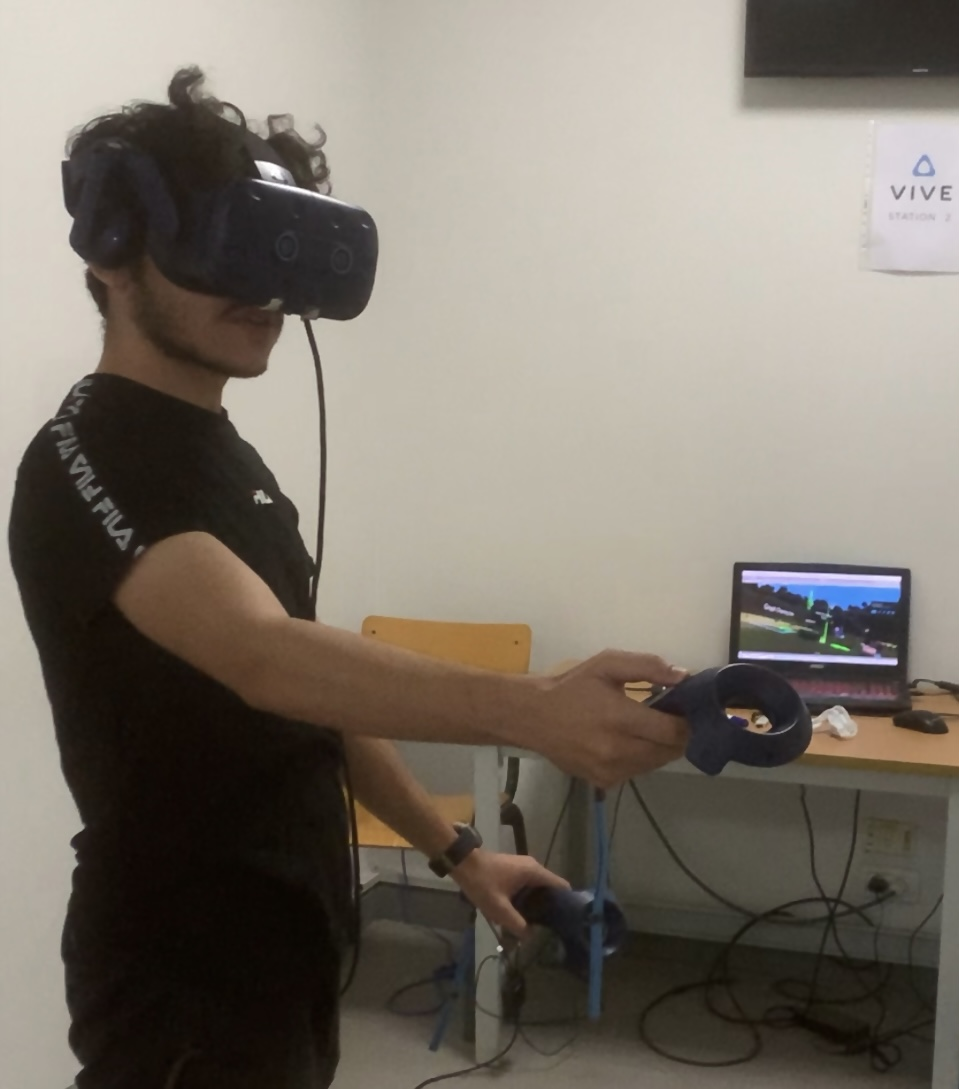
\includegraphics[width=0.8\textwidth]{images/participant1.png}
    \end{minipage}
    \begin{minipage}{0.45\textwidth}
        \centering
        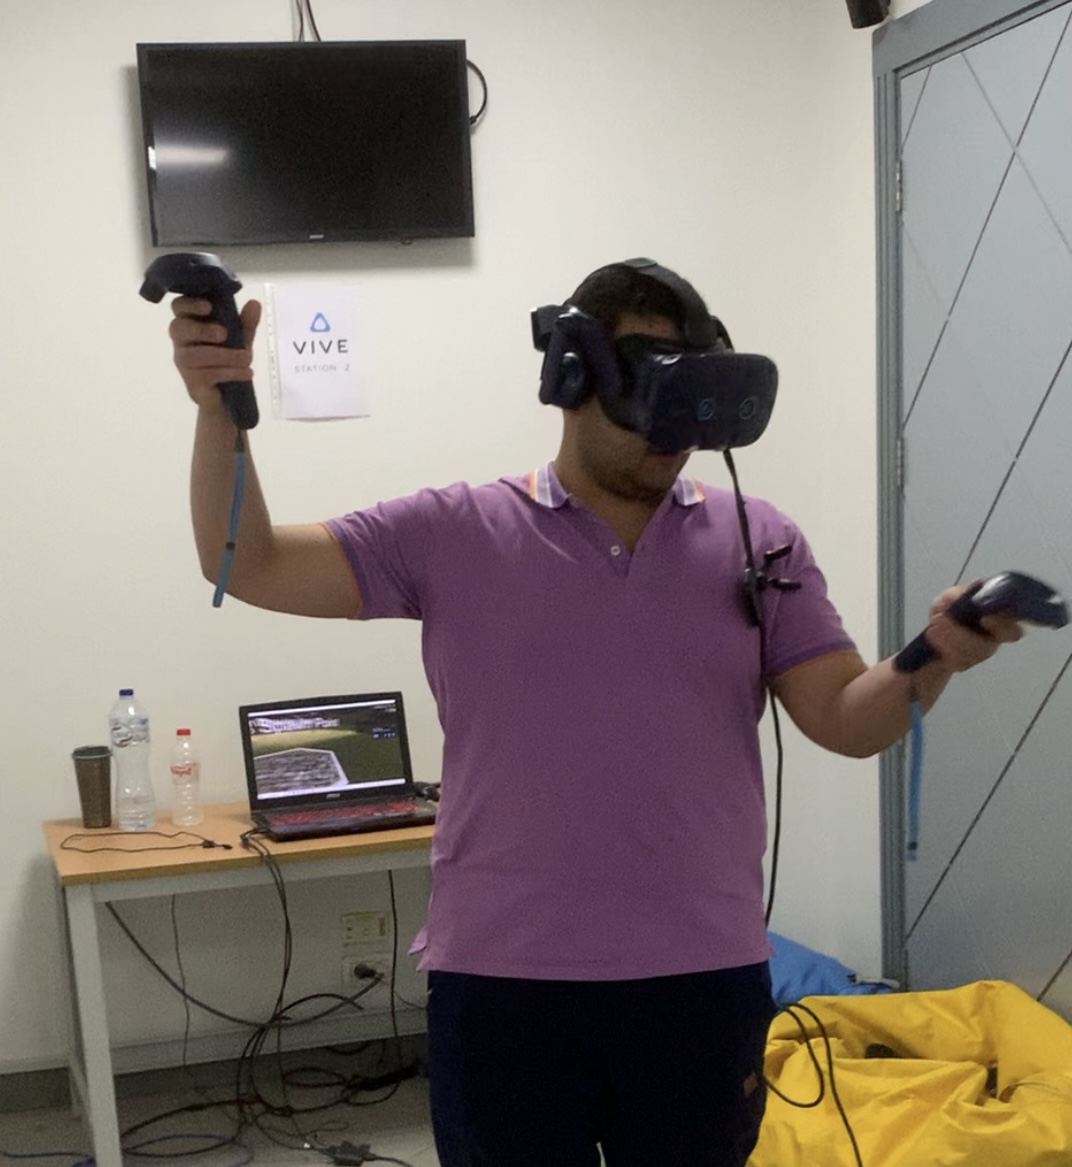
\includegraphics[width=0.8\textwidth]{images/participant2.PNG}
    \end{minipage}
    \captionsetup{justification=centering}
    \caption[]{Participants in the test session}

\end{figure}

\subsection{Survey} \label{sec:survey}
After the test session, the participants were asked to fill out a survey to provide feedback on their experience. The survey included questions about the participants' understanding of the \ac{POP} algorithm, their experience with the \ac{VR} environment in the test session, and a \ac{SUS} questionnaire to evaluate the usability of the system. The survey was conducted using Google Forms to be easily accessible to the participants.

\subsubsection{Feedback Questions} \label{sec:feedback_questions}
The survey included the following questions to gather feedback from the participants:
\begin{enumerate}
    \item I think the VR game helped me to understand the POP Algorithm more (than theoretically). \textit{(10-point Likert scale)}
    \item I felt the VR game made the algorithm more interesting or engaging. \textit{(5-point Likert scale)}
    \item I would recommend the game as a learning tool to others. \textit{(5-point Likert scale)}
\end{enumerate}


\subsubsection{System Usability Scale (SUS)}
The \ac{SUS} is a widely used questionnaire for evaluating the usability of a system. The questionnaire consists of 10 questions, each with a 5-point Likert scale. The scores of the odd-numbered questions are subtracted by 1, and the scores of the even-numbered questions are subtracted from 5. The scores are then summed up and multiplied by 2.5 to get the final \ac{SUS} score, which ranges from 0 to 100. The \ac{SUS} score is used to evaluate the usability of the system, with higher scores indicating better usability. An average \ac{SUS} score is considered to be 68 \cite{SUSmeasure}. The \ac{SUS} questionnaire is shown in \autoref{fig:sus}.
\begin{lstlisting}[ frame=single, basicstyle=\small\ttfamily, breaklines=true, captionpos=b,caption={System Usability Scale (SUS) Questionnaire},label={fig:sus}]
    1. I think that I would like to use this system frequently.
    2. I found the system unnecessarily complex.
    3. I thought the system was easy to use.
    4. I think that I would need the support of a technical person to be able to use this system.
    5. I found the various functions in this system were well integrated.
    6. I thought there was too much inconsistency in this system.
    7. I would imagine that most people would learn to use this system very quickly.
    8. I found the system very cumbersome to use.
    9. I felt very confident using the system.
    10. I needed to learn a lot of things before I could get going with this system.    
\end{lstlisting}





\section{Results}

The results of the evaluation process are presented in this section. The results include the participants' feedback on the \ac{POP} algorithm and the \ac{VR} environment, as well as the results of the \ac{SUS} questionnaire.

\subsection{Participants' Feedback}

The participants' feedback on the \ac{POP} algorithm and the \ac{VR} environment was collected through the survey. The participants were asked to rate their understanding of the \ac{POP} algorithm, the effectiveness of the \ac{VR} environment in enhancing their understanding of the algorithm, and the engagement level of the \ac{VR} environment. The participants were also asked if they would recommend the game as a learning tool to others. The results of the feedback questions, that are listed in the \textit{Feedback Questions} in \autoref{sec:feedback_questions}, are shown in \autoref{fig:feedback}.

The results show that the majority of the participants found the \ac{VR} environment helpful in understanding the \ac{POP} algorithm. More than 90\% of the participants answered 7 or above on the 10-point Likert scale question. The participants also found the \ac{VR} environment engaging, with 95\% of the participants answering 4 or above on the 5-point Likert scale question. Finally, 90\% of the participants answered 4 or above and said they would recommend the game as a learning tool to others. These results indicate that the \ac{VR} environment was effective in enhancing the participants' understanding of the \ac{POP} algorithm and engaging them in the learning process. Moreover, in the open-ended feedback section, the participants expressed their satisfaction with the \ac{VR} environment and the learning experience, and provided suggestions for improvement, which will be considered and added in the future work section.

\begin{figure}
    \centering
    \begin{minipage}{0.45\textwidth}
        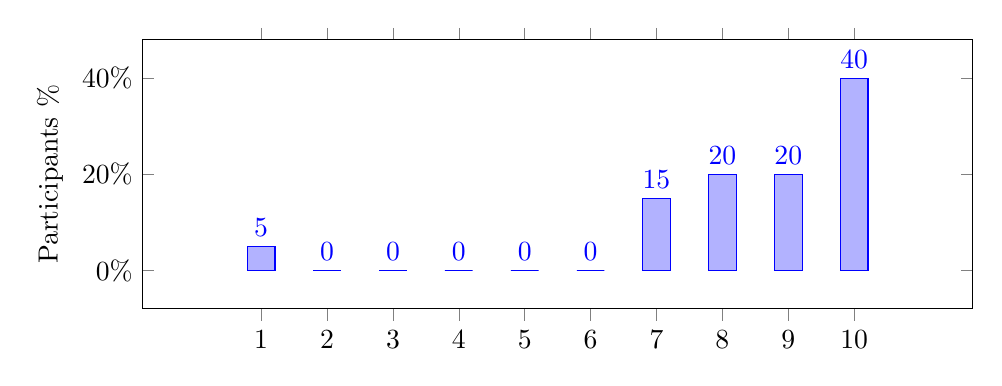
\begin{tikzpicture}
            \begin{axis}[
                    width=\textwidth,
                    height=5cm,
                    ybar,
                    enlargelimits=0.2,
                    legend style={at={(0.5,-0.15)},
                            anchor=north,legend columns=-1},
                    ylabel={Participants \%},
                    symbolic x coords={1,2,3,4,5,6,7,8,9,10},
                    xtick=data,
                    nodes near coords,
                    nodes near coords align={vertical},
                    yticklabel={\pgfmathprintnumber{\tick}\%},
                ]
                \addplot coordinates {(1,5) (2,0) (3,0) (4,0) (5,0) (6,0) (7,15) (8,20) (9,20) (10,40)};
            \end{axis}
        \end{tikzpicture}
    \end{minipage}
    \begin{minipage}{0.26\textwidth}
        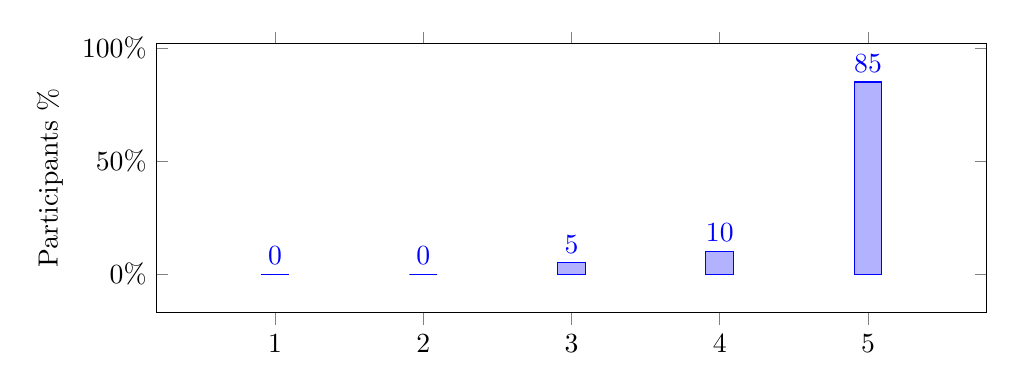
\begin{tikzpicture}
            \begin{axis}[
                    width=\textwidth,
                    height=5cm,
                    ybar,
                    enlargelimits=0.2,
                    legend style={at={(0.5,-0.15)},
                            anchor=north,legend columns=-1},
                    ylabel={Participants \%},
                    symbolic x coords={1,2,3,4,5},
                    xtick=data,
                    nodes near coords,
                    nodes near coords align={vertical},
                    yticklabel={\pgfmathprintnumber{\tick}\%},
                ]
                \addplot coordinates {(1,0) (2,0) (3,5) (4,10) (5,85)};
            \end{axis}
        \end{tikzpicture}
    \end{minipage}
    \begin{minipage}{0.26\textwidth}
        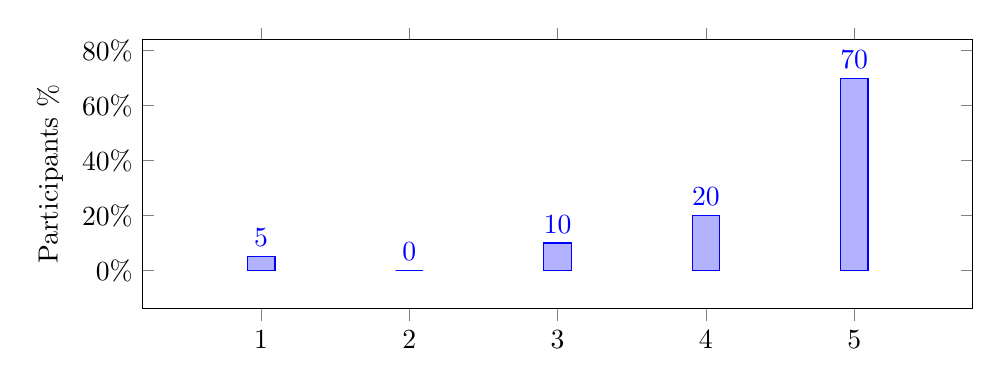
\begin{tikzpicture}
            \begin{axis}[
                    width=\textwidth,
                    height=5cm,
                    ybar,
                    enlargelimits=0.2,
                    legend style={at={(0.5,-0.15)},
                            anchor=north,legend columns=-1},
                    ylabel={Participants \%},
                    symbolic x coords={1,2,3,4,5},
                    xtick=data,
                    nodes near coords,
                    nodes near coords align={vertical},
                    yticklabel={\pgfmathprintnumber{\tick}\%},
                ]
                \addplot coordinates {(1,5) (2,0) (3,10) (4,20) (5,70)};
            \end{axis}
        \end{tikzpicture}
    \end{minipage}
    \captionsetup{justification=centering}
    \caption[]{Participants' response on the POP algorithm and the VR environment Feedback Questions 1, 2, and 3 respectively}
    \label{fig:feedback}
\end{figure}

\subsection{System Usability Scale (SUS) Results}
% Standard Deviation	s =	11.363463
% Variance	s2 =	129.12829
% Count	n =	20
% Mean	x¯¯¯
%  =	79.125
% Sum of Squares	SS =	2453.4375

The results of the \ac{SUS} questionnaire are shown in \autoref{fig:sus_results}. The average \ac{SUS} score was 79.125, which is higher than the average \ac{SUS} score of 68. This indicates that the \ac{VR} environment had good usability, and the participants found it easy to use and engaging. The standard deviation of the \ac{SUS} score was 11.363, which indicates that the participants' opinions were not significantly high or low, and the variance was 129.128, which indicates that the participants' opinions were not significantly different from each other.



\begin{figure}[H]
    \centering
    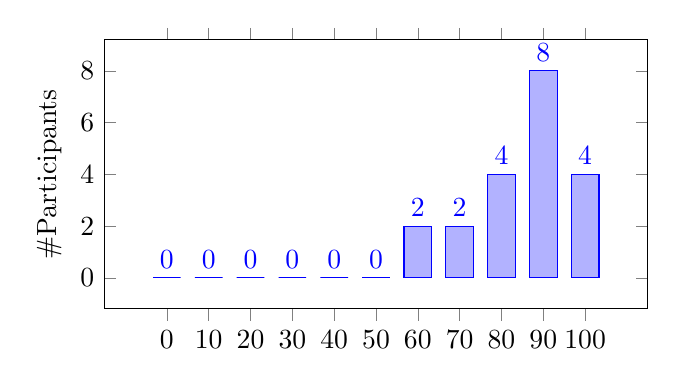
\begin{tikzpicture}
        \begin{axis}[
                width=0.7\textwidth,
                height=5cm,
                ybar,
                enlargelimits=0.15,
                legend style={at={(0.5,-0.15)},
                        anchor=north,legend columns=-1},
                ylabel={\#Participants},
                symbolic x coords={0,10,20,30,40,50,60,70,80,90,100},
                xtick=data,
                nodes near coords,
                nodes near coords align={vertical},
                yticklabel={\pgfmathprintnumber{\tick}},
            ]
            \addplot coordinates {(0,0) (10,0) (20,0) (30,0) (40,0) (50,0) (60,2) (70,2) (80,4) (90,8) (100,4)};
        \end{axis}
    \end{tikzpicture}
    \captionsetup{justification=centering}
    \caption[]{Participants' response on the System Usability Scale (SUS) Questionnaire}
    \label{fig:sus_results}
\end{figure}

\section{Discussion}

The results of the evaluation process indicate that the \ac{VR} environment was effective in enhancing the participants' understanding of the \ac{POP} algorithm and engaging them in the learning process. The majority of the participants found the \ac{VR} environment helpful in understanding the algorithm, engaging, and would recommend the game as a learning tool to others. The \ac{SUS} score of 79.125 indicates that the \ac{VR} environment had good usability, and the participants found it easy to use. The participants' feedback and the \ac{SUS} score show that the \ac{VR} environment was successful in enhancing the learning effectiveness of the \ac{POP} algorithm and providing an engaging learning experience.